\section{Results}

\subsection{Code availability}

All the code for TorchIO is available on GitHub\fnurl{https://github.com/fepegar/torchio}.
We follow the semantic versioning system \cite{preston-werner_semantic_2020} to tag and release our library.
Releases are published on the Zenodo data repository\fnurl{https://zenodo.org/} to allow users to cite the specific version of the package they used in their experiments.
The version described in this paper is \torchioversion \cite{perez-garcia_fepegartorchio_2020}.
Detailed \ac{API} documentation is hosted on Read the Docs and comprehensive Jupyter notebook tutorials are hosted on Google Colaboratory, where users can run examples online.
The library can be installed with a single line of code on Windows, macOS or Linux using the \ac{PIP} package manager: \texttt{pip install torchio}.

TorchIO has a strong community of users, with more than 1100 stars on GitHub and more than 2000 \ac{PyPI} downloads per week\fnurl{https://pypistats.org/packages/torchio} as of October 2021.


\subsubsection{Additional interfaces}

The provided \ac{CLI} tool \texttt{torchio-transform} allows users to apply a transform to an image file without using Python.
This tool can be used to visualize only the preprocessing and data augmentation pipelines and aid in experimental design for a given application.
It can also be used in shell scripts to preprocess and augment datasets in cases where large storage is available and on-the-fly loading needs to be faster.

Additionally, we provide a \ac{GUI} implemented as a Python scripted module within the \textit{TorchIO} extension available in 3D Slicer~\cite{fedorov_3d_2012}%
\fnurl{https://github.com/fepegar/SlicerTorchIO}.
It can be used to visualize the effect of the transforms parameters without any coding (\cref{fig:slicer}).
As with the \ac{CLI} tool, users can experimentally assess preprocessing and data augmentation before network training to ensure the preprocessing pipeline is suitable for a given application.

\begin{figure}
  \centering
  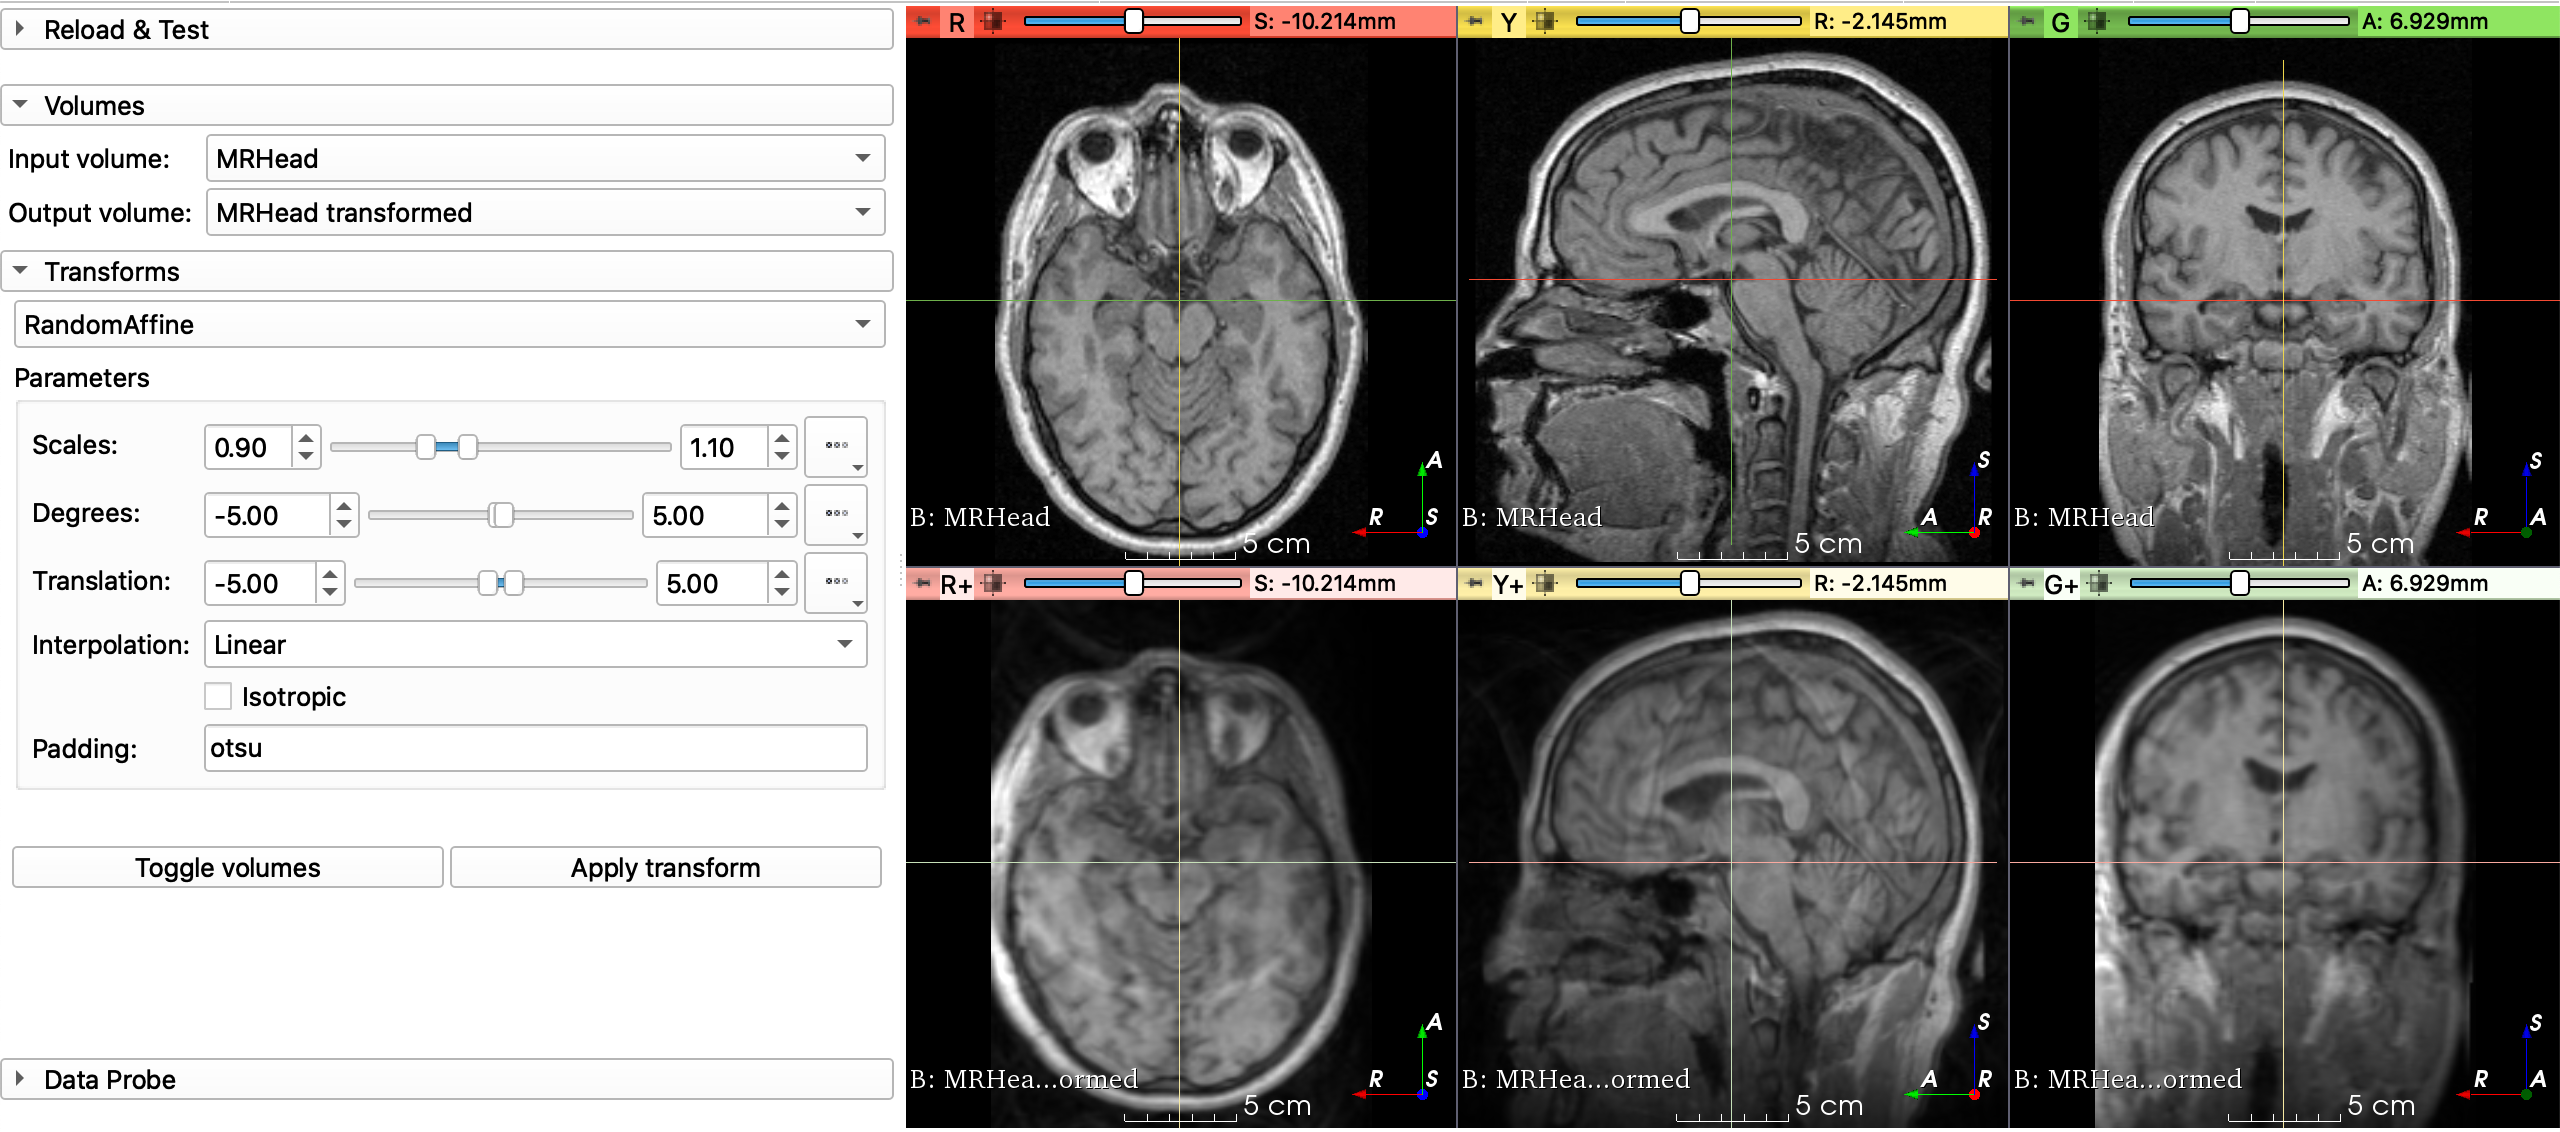
\includegraphics[width=\linewidth, trim = {0 0 0 0.1cm}, clip]{slicer}
  \caption[Graphical user interface for TorchIO]{
    \Ac{GUI} for TorchIO, implemented as a 3D Slicer extension.
    In this example, the applied transforms are
    \texttt{RandomBiasField},
    \texttt{RandomGhosting},
    \texttt{RandomMotion},
    \texttt{RandomAffine} and
    \texttt{RandomElasticDeformation}.
  }
  \label{fig:slicer}
\end{figure}
